\chapter{IoT}
Internet delle cose (Internet of Things, IoT) è un paradigma riferito
all’estensione di internet al mondo degli oggetti. Questo concetto è stato
introdotto nel 1999 da Kevin Ashton, ricercatore britannico del Mit
(Massachusetts Institute of Technology), che teorizzò per primo un mondo nel
quale oggetti dotati di sensori, interagiscono utilizzando la rete.  La continua
evoluzione delle tecnologie wireless e satellitari ha permesso l'ideazione di
oggetti sempre più connessi, in grado di generare una mole di informazioni e
dati.  Non sono dunque, come tradizionalmente si potrebbe pensare, solo computer
o tablet ad essere connessi alla rete, ma anche gli oggetti che usiamo
quotidianamente , che divenendo “smart” riescono a fornire al utente
applicazioni facili da usare.  Ad esempio gli smart watch o smart band che
monitorano il jogging quotidiano, il quale  fornisce informazioni riguardanti il
numero di chilometri percorsi, la velocità media ecc sfruttando il Gps (Global
Positioning System) in maniera autonoma senza doversi appoggiare a un computer.
La presenza negli oggetti di sensori connessi alla rete (e agli altri oggetti
smart) permette un trasferimento di dati bidirezionale tra l'oggetto stesso ed
il server al quale questi dati vengono inviati.  L'oggetto infatti dopo aver
trasformato in dati gli input ricevuti dall'ambiente esterno, invia queste
informazioni ad un serve il quale, dopo un'elaborazione degli stessi, formula
dei comandi da inviare all'oggetto.  Nel mondo dell’IoT i dati condivisi sono in
continuo aumento, innescando una serie di progressi importanti anche da un punto
di vista economico, andando ad incidere  significativamente sulla “catena del
valore” (value chain). Attraverso lo studio delle informazioni presenti si
potranno andare a creare applicazioni in grado di aumentare l’efficienza di un
servizio, migliorare la user experience di una applicazione ecc.  Muovendoci
verso un modo sempre più connesso, nove problematiche riguardanti la privacy e
la sicurezza emergo.  Molto spesso per ridurre i costi di produzione e di
sviluppo di questi oggetti smart, Numerosi attacchi hacker si sono già verificati andando a
sfruttare le falle di sicurezza di questi oggetti "smart" 
\section{La tecnologia alla base dell'IoT} 
Come detto in precedenza, nel mondo industriale il concetto di poter connettere
oggetti per ricevere informazioni utili non è nuovo. Nel corso degli anni le
tecnologie alla base di questo paradigma si sono evolute, rendendo sempre più
autonomi e "smart" gli oggetti a esse collegati. Tag RFID , codici QR, ZigBee,
sono gli "arti" del sistema IoT. La spina dorsale di questo mondo è composta da
una architettura bottom up suddivisa in tre livelli.
\begin{itemize}
\item \textbf{Device layer} o sensor layer, è il layer più basso. Esso raggruppa
tutti i gli oggetti "smart". Questo layer è quello che mette in comunicazione il
mondo reale con gli atri layer superiori. A loro spetta lo scopo di convertire
una misura fisica in un segnale interpretabile da altri calcolatori.
La maggior parte di questi sensori, utilizzerà una connessione Bluetooth,
ZigBee, Wifi o una si baserà su una rete LPWAN per comunicare il dato al layer
superiore.
\item \textbf{Network layer} o mediation layer raggruppa l'intera infrastruttura
di rete e gateway che ricevono i dati da i vari sensori. Questo layer è
semplicemente un layer di mediazione dove l'informazione (dato) non viene altera
ma semplicemente trasmesso all'Application layer.
\item \textbf{Application layer} è il layer nel quale l'informazione viene
immagazzinata ed elaborata. Questo layer è il più importante, e qui dove il dato
viene trasformato da una semplice misurazione fisica ad una possibile revenue
per l'azienda che lo gestisce.\improvement{Riscrivere}
\end{itemize}
\section{La diffusione dell'Internet delle cose}
Nel 2008 il numero di oggetti quali computer, telefoni cellulari, table,
connessi ad internet ha superato il numero di persone presenti nell'intero
pianeta. Il continuo sviluppo tecnologico ha portato all'abbassamento del costo
del hardware stesso. Secondo  una stima da parte di Gartner, il numero di smart device sarà
superiore a 20 miliardi \ref{gartner2016}
\begin{figure}[h]
        \centering 
                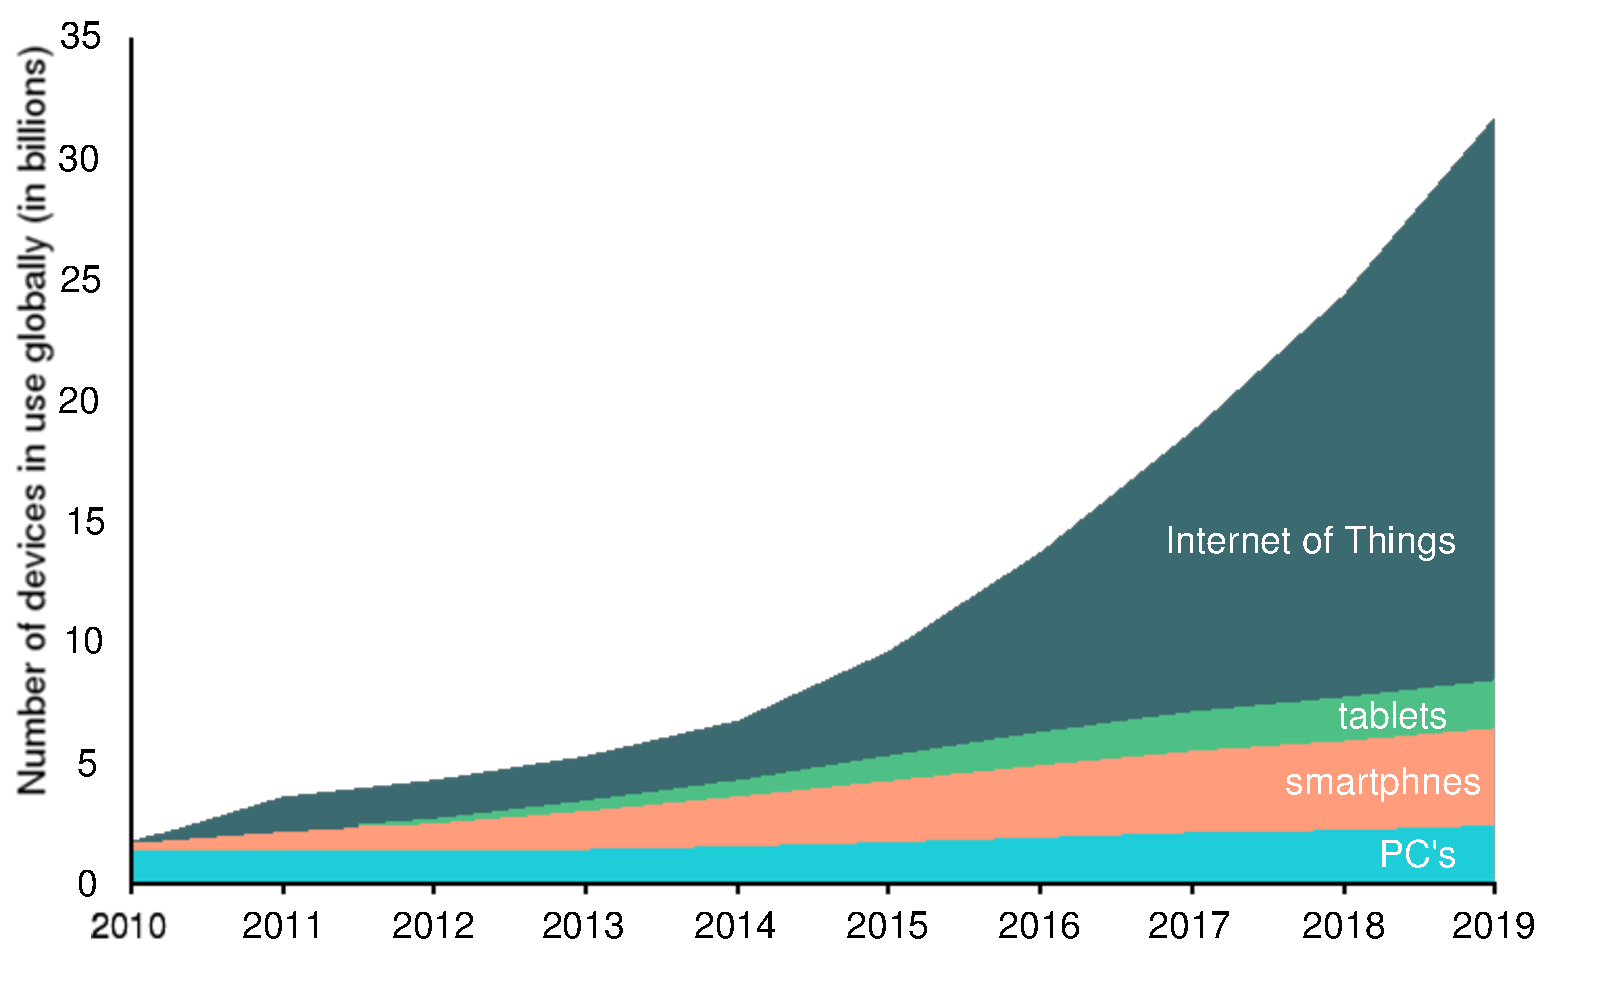
\includegraphics[width=10cm]{iot_devices}
        \caption{Numero di dispositivi per anno}
\end{figure}

\section{Big Data}
Oltre all'innumerevole quantità di dati che verrà prodotta da questi milioni di
devices intelligenti, noi stessi, facendo ricerche su siti internet e navigando
nel web produciamo una grande quantità di dati. Il termine Big Data è nato per
rappresentare l'insieme di tutti i dati eterogenei che ogni giorno vengono
prodotti e scambiati nella rete.
In questo contesto riuscire ad estrapolare l'informazione utile diventa sempre
più difficile. Con il progredire della tecnologia il dataset (aggregazione di
dati) a disposizione delle aziende è in continuo aumento. Aziende ed enti
pubblici stanno investendo e mettendo a disposizione sempre più servizi in grado
di usufruire in maniera efficace dei dati raccolti. Secondo un articolo
pubblicato da Verizon, si stima che il 92\% delle aziende usa meno del 25\% dei
dati raccolti e che solo il 50\% di esse prevede di riuscire a fare fruttare più
del 25\% di dati nei prossimi due anni \cite{Verizon}.
Il "carburante" dell'IoT sono i dati raccolti, sono loro a il valore
valore aggiunto. Per le aziende pubbliche e private, l'informazione ha
sempre rappresentato una risorsa economica su cui investire. Riuscire a
prevedere i nuovi trend del mercato e a stimare con precisione le vendite dei
mesi futuri in maniera esatta è sempre stato l'obbiettivo preposto dall'analista
di mercato.
Grazie all'innumerevole quantità di dati che noi produciamo semplicemente
navigando il web 
Al giorno d'oggi sempre più spesso sentiamo parlare di industria 4.0, ovvero il
riuscire ad elaborare la grande quantità di dati che vengono creati, per andare
a riutilizzarli nel ambito aziendale, migliorando la qualità dei prodotti ed
aumentare la produttività dell'azienda stessa .
 
Un termine spesso è presente quando si parla di IoT è il
termine Big Data. Con Big Data si intende tutte 
Come un’automobile necessita di benzina per funzionare, così l’IoT necessita di
dati per alimentarsi e migliorarsi. Due ambiti diversi ma connessi che combinati
producono una sorta di “superpotere” nelle mani di soggetti pubblici e aziende.
Soprattutto per queste ultime, l’informazione da sempre ha rappresentato una
risorsa economica e saper analizzare i dati raccolti dagli oggetti smart appare
essere una vera e propria sfida da cogliere senza esitazione alle porte dell’economia
2.0. Il data mining si afferma come uno dei settori più strategici per le aziende che
operano nel contesto contemporaneo, le quali, autonomamente o grazie all’aiuto di
esperti, possono incrociare dati avendo l’utente come unità di analisi per scoprire
opportunità di investimenti economici enormi. Ma cosa sono i dati e come si arriva
ai megadati (big data) è argomento tutt’ora dibattuto.
Un problema trasversale che interessa gli esperti di diritto e non solo, è quanto
concerne la definizione di “dato” e di “dato personale”. Infatti, oggigiorno, ci sono
norme che si applicano per i “dati” e norme che si applicano per i “dati personali”
e più specificatamente per i “dati sensibili”. Altro problema che fa discutere è se
rientrino nei “dati” anche i cosiddetti “metadati”, ovvero quelle informazioni che
associate ad una pagina web, o anche ad una parte di essa, riescono a descriverne
il contenuto e il contesto di riferimento 13 .
Seguendo le linee guida Ocse del 1980, rivedute nel 2013 14 , sono da definirsi come
“dati personali” tutte quelle informazioni relative ad un determinato individuo 15 e
che possono fornire dettagli sulle sue caratteristiche, le sue abitudini, il suo stile
di vita, il suo stato di salute, ecc. A questa definizione, ripresa anche dalla Direttiva
95/46/CE del 1995 16 , segue quella di “dato sensibile” riportata anche dal Codice in
